\documentclass{article}
\usepackage[utf8]{inputenc}
\title{video 5: CONFIDENCE INTERVALS FOR PROBABILITIES AND PROPORTIONS}
\author{wbg231 }
\date{December 2022}
\newcommand{\R}{$\mathbb{R}$}
\newcommand{\B}{$\beta$}
\newcommand{\A}{$\alpha$}
\newcommand{\D}{\Delta}

\newcommand{\avector}[2]{(#1_2,\ldots,#1_{#2})}
\newcommand{\makedef}[2]{$\textbf{#1}$:#2 }
\usepackage{tikz,graphicx,hyperref,amsmath,amsfonts,amscd,amssymb,bm,cite,epsfig,epsf,url}

\begin{document}

\maketitle

\section*{introduction}
\begin{itemize}
\item \href{https://www.youtube.com/watch?v=dlGl2dGNZSI}{video link}
\section{motivating example}
\item suppose we are the government and want to get an idea of the percentage of people with covid 19 
\item we can not test the whole population, so we can only take a sample 
\item and the fraction of people that test positive will be our estimate of the population prevalence 
\item even though the population prevalence will not change, if we take a different sample our estimate of the prevalence will change 
\item so we want to use confidence intervals to understand this uncertainty
\section{confidence interval for proportion}
\subsection{confidence interval}
\item the idea is instead of just reporting our estimate we also report a range of values that contain the population parameter with a probability of $(1-\alpha)$
\subsection{sample proportion }
\item we have data $a_1...a_n$ taking value 1 to indicate if a person has covid and 0 otherwise
\item we take random samples from  this data $\Tilde{x}_1...\Tilde{x}_n$ randomly and independently
\item in this case the sample proportion is the mean of our measurements 
\subsection{confidence interval for the mean}
\item this means we can use the confidence interval for mean we built last video for the sample proportion
\item the population population mean is $\mu_{pop}$ and population variance is $\sigma_{pop}^{2}$
\item random samples are selected independently and uniformly at random with replacement $\Tilde{x}_1...\Tilde{x}_n$ from the population. 
\item the sample mean $\Tilde{m}=\frac{1}{n}\Sigma_{i=1}^{n}\Tilde{x}_{i}$
\item $E[m]=\mu$ and sample mean is unbiased
\item $se(m)=\frac{\sigma}{\sqrt{n}}$ that is the standard error of the sample mean is decreasing in n 
\item further we know that as $n\rightarrow \infty$ $\Tilde{m}_{n}$ converges in distribution to a Gaussian with mean $\mu_{pop}$ and variance $se(\Tilde{m}))=\frac{1\sigma}{\sqrt{n}}$
\item so then assuming that the sample mean is Gaussian which holds for really large values of n we can write $\Tilde{\mathcal{I}}_{1-\alpha}=[\Tilde{m}-c_{\alpha}se(m),\Tilde{m}+c_{\alpha}se(m)]=[\Tilde{m}-\frac{c_{\alpha}\sigma_{pop}}{\sqrt{n}},\Tilde{m}+\frac{c_{\alpha}\sigma_{pop}}{\sqrt{n}}]$ where  $c_{\alpha}=F_\Tilde{z}^{-1}(1-\frac{\alpha}{2})$
\item so lets apply this to a sample proportion 


\subsection{confidence interval for a probability}
\item if $\Tilde{b}_1...\Tilde{b}_{n}$ Are Bernoulli rv with parameter $\theta$
\item then the sample proprietor is  is $\Tilde{m}-\frac{1}{n}\Sigma_{i=1}^{n}\Tilde{b}_i$
\item we know that $E[m]=\theta$
\item we know that $var(m)=\frac{\tehta(1-\theta)}{m}$ by Independence 
\tiem then by the central limit theorem we can write our confiding interval as 
$\Tilde{\mathcal{I}}_{1-\alpha}=[\Tilde{m}-c_{\alpha}se(m),\Tilde{m}+c_{\alpha}se(m)]=[\Tilde{m}-c_{\alpha}\sqrt{\frac{\theta(1-\theta)}{n}},\Tilde{m}+c_{\alpha}\sqrt{\frac{\theta(1-\theta)}{n}}]$ where  $c_{\alpha}=F_\Tilde{z}^{-1}(1-\frac{\alpha}{2})$ 
\item here an issue is we do not know $\theta$ but we know that $\theta\in[0,1]$ since it is a probability

\subsection{bounding confiding interval for probability}
\item lets think about bounding our interval
\item $\Tilde{\mathcal{I}}_{1-\alpha}==[\Tilde{m}-c_{\alpha}\sqrt{\frac{\theta(1-\theta)}{n}},\Tilde{m}+c_{\alpha}\sqrt{\frac{\theta(1-\theta)}{n}}]$
\item $h(\theta)=\theta(1-\theta)$ has derivative $1-2\theta$ and second derivative $-2$ so $\theta^{*}=\frac{1}{2}$ in other words we know the max value of h occurs when $\theata=$ $\frac{1}{2}$ and it will be $\h(\theta)=\frac{1}{2}\frac{1}{2}=\frac{1}{4}$
\item in other words $h(\theta)$ is upper bounded by 1 fourth so we can set our $h(\theta)=\frac{1}{4}$ and have the most conservative confidence interval
\item so we can write our interval as $\Tilde{\mathcal{I}}_{1-\alpha}==[\Tilde{m}-c_{\alpha}\sqrt{\frac{1}{4n}},\Tilde{m}+c_{\alpha}\sqrt{\frac{1)}{4n}}]=[\Tilde{m}-\frac{.5c_{\alpha}}{\sqrt{n}},\Tilde{m}+\frac{.5c_{\alpha}}{\sqrt{n}}]$ 
\item so by choosing this width to be the upper bound we know, it will be valid regardless of the variance of the data.
\subsection{confidence interval for population proportion }
\item we have data $a_1...a_n$ taking value 1 to indicate if a person has covid and 0 otherwise
\item we take random samples from  this data $\Tilde{x}_1...\Tilde{x}_n$ randomly and independently
\item they are Bernoulli with parameter $\theta_{pop}$
\item thus we can construct a confidence interval as $\Tilde{\mathcal{I}}_{1-\alpha}=[\Tilde{m}-\frac{.5c_{\alpha}}{\sqrt{n}},\Tilde{m}+\frac{.5c_{\alpha}}{\sqrt{n}}]$ 
\item so we can use this to calculate an n such that our sample proportion will have a certain error (that is our confidence interval will have a width)
\item so if we want an error $\leq 1\%$ then we need $\frac{.5c_{\alpha}}{\sqrt{n}}\leq 1\Rightarrow n\geq (\frac{c_{\alpha}}{.01})^2$
\section{monte carlo method}
\subsection{monte carlo method}
\item we want to estimate $p(a)$ by simulating outcomes and choking how many we observe
\item the key question is how many simulations are enough 
\item we can use confidence intervals to get a bound on how many simulations we need 
\subsection{example}
\item Tokyo Olympics 3X3 basketball tournament what is the likelihood that each team wins? we are simulating with monte carlo methods 
\item to estimate the  portability that a team wins is $\theta$
\item we simulate the tournament n times independently 
\item where in each simulation P(team wins)=$\theta$
\item then we compute the fraction of simulations in which the team wins 
\item this gives us the sample mean of n Bernoulli random variables with parameter $\theta$
\item $\Tilde{\mathcal{I}}_{1-\alpha}=[\Tilde{m}-\frac{.5c_{\alpha}}{\sqrt{n}},\Tilde{m}+\frac{.5c_{\alpha}}{\sqrt{n}}]$ 
\subsection{results }
\item after 1000 simulations we can construct confidence intervals for our estimate of the likelihood of each team winning 
\item 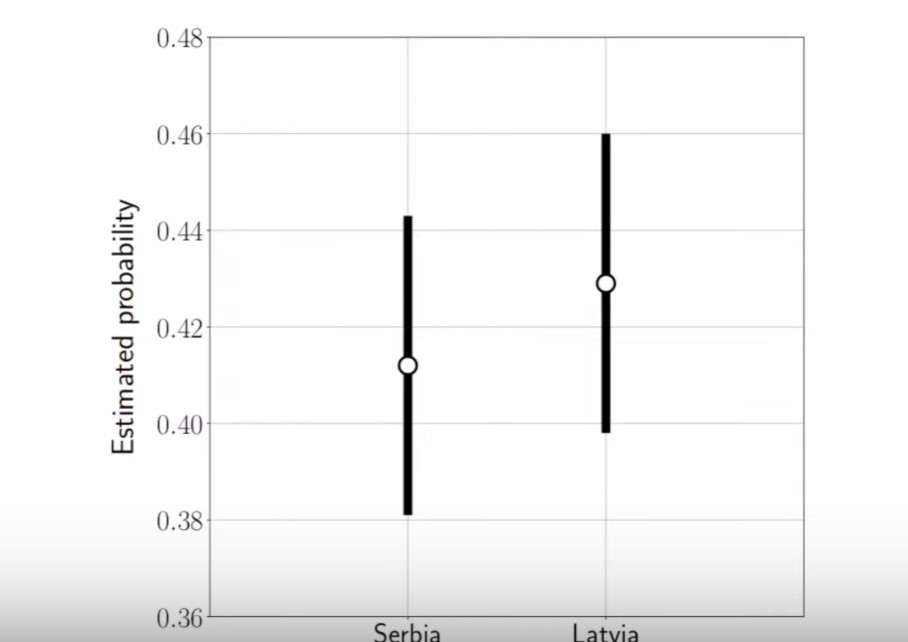
\includegraphics[width=10cm]{notes/week_4/vidio 5:CONFIDENCE INTERVALS FOR PROBABILITIES AND PROPORTIONS/immages/v4_4.jpg}
\item notice that our confidence intervals are overlapping this means that based on our estimate there is a more than $\alpha\%$ chance we got it wrong, that is we can not be sure that one team wins more often than another 
\item so we can increase n until we are sure that the confidence intervals do not overlap 
\item  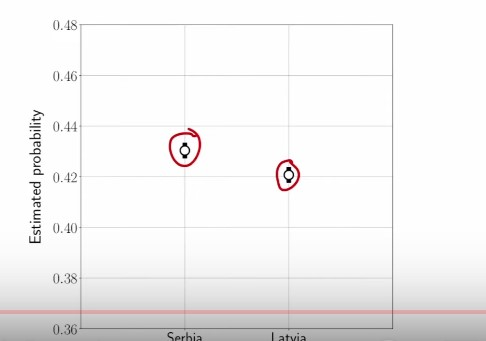
\includegraphics[width=10cm]{notes/week_4/vidio 5:CONFIDENCE INTERVALS FOR PROBABILITIES AND PROPORTIONS/immages/v4_5.jpg}
\item this is how we use confidence intervals to ensure we have preformed enough monte carlo simulations 
\section{polling example}
\item in a pool 281 people vote for Biden 300 for trump 
\item let $\theta$ be the fraction for people who plan to vote for trump
\item then we can construct a ci as \item $\Tilde{\mathcal{I}}_{1-\alpha}=[\Tilde{m}-\frac{.5c_{\alpha}}{\sqrt{n}},\Tilde{m}+\frac{.5c_{\alpha}}{\sqrt{n}}]$ and calculate the confidence interval with our actual sample mean and n and get [.44,.52]
\item we are producing the outcome of an election, so we are really interested in $P(\theta\geq .5)$
\item but our confidences interval tells us nothing about $P(\theta\geq .5)$ but here we are treating $\theta$ as deterministic, so we can not make any statements about if he will win or not 
\item we can do this with a Bayesian frame work though, but we need a prior distribution of $\theta$
\section{if assumptions are violated}
\item we are assuming Independence of our random samples if this is violated then our confidence intervals are not valid .
\item so if we are trying to estimate the average rain fall in an area, and we chose to pick data points just from the month of April.
\item it tends to train more in that month than average so the samples are not independent and our ci is not valid
\item if we do no random sampling over the year our ci can still be descriptive
\item so our assumptions of Independence and uniform sampling must be valid for our ci to be valid  
\end{itemize}
\end{document}
